\chapter{Parameter learning}\label{chp:weights}

The objective of this chapter is to expose the ideas behind generative and discriminative gradient
descent for parameter learning of sum-product networks. We first show how to derive the SPN with
respect to its nods and weights so that we can find the gradient of the SPN wrt its parameters
(i.e.\ weights). This allows us to find the weight updates needed for gradient descent on SPNs. We
then describe how to perform generative stochastic gradient descent, and finally discriminative
gradient descent.

\section{Derivatives}

Let $S$ be an SPN\@. We are only interested in finding the derivative of internal nodes, as leaf
nodes have no weights to be updated. Our objective is to find the gradient $\iddspn{S}{W}$ by
computing each component $\iddspn{S}{w_{n,j}}$, allowing us to find each weight update on the
SPN\@.

At each weighted edge $(n\to j, w_{n,j})$, the derivative $\iddspn{S}{w_{n,j}}$ takes the form

\begin{equation}
  \ddspn{S}{w_{n,j}}(X)=\ddspn{S}{S_n}\ddspn{S_n}{w_{n,j}}(X)=
    \ddspn{S}{S_n}\ddspn{}{w_{n,j}}\left(\sum_{i\in\Ch(n)}w_{n,i}S_i(X)\right)=
    \ddspn{S}{S_n}S_j(X).
\end{equation}

The term $\iddspn{S}{S_n}$ appears because of chain rule, since $S_n$ is a function of $S$. This
can be intuitively interpreted as taking into account the change in all nodes ``above'' $n$. So to
compute the derivative wrt a weight, we need to find the derivative $\iddspn{S}{S_j}$ for each
internal node $j$.

Finding $\iddspn{S}{S_j}$ requires analyzing two possible cases: sum and product parents of $j$.
We now that $S$ is a multilinear function of $X$, since in reality $S$ is just a function made of
sums and products. In particular, if we apply chain rule on $\iddspn{S}{S_j}$, we have that

\begin{equation*}
  \ddspn{S}{S_j}(X)=\underbrace{\sum_{\substack{n\in\Pa(j)\\n:\text{
          sum}}}\ddspn{S}{S_n}\ddspn{S_n}{S_j}(X)}_{(\ast)}+
    \underbrace{\sum_{\substack{n\in\Pa(j)\\n:\text{
            product}}}\ddspn{S}{S_n}\ddspn{S_n}{S_j}(X).}_{(\ast\ast)}
\end{equation*}

We expand each term at a time. Starting with the sum parents case, we can substitute the value of
$S_n(X)$ with the corresponding expansion.

\begin{equation*}
  (\ast)=\sum_{\substack{n\in\Pa(j)\\n:\text{ sum}}}\ddspn{S}{S_n}\ddspn{}{S_j}\left(\sum_{i\in\Ch(n)}
    w_{n,i}S_i(X)\right)=\sum_{\substack{n\in\Pa(j)\\n:\text{ sum}}}\ddspn{S}{S_n}w_{n,j}
\end{equation*}

We do the same for the product case.

\begin{equation*}
  (\ast\ast)=\sum_{\substack{n\in\Pa(j)\\n:\text{ product}}}\ddspn{S}{S_n}\ddspn{}{S_j}\left(\prod_{i\in\Ch(n)}
    S_i(X)\right)=\sum_{\substack{n\in\Pa(j)\\n:\text{ product}}}\ddspn{S}{S_n}\prod_{k\in
      \Ch(n)\setminus\{j\}}S_k
\end{equation*}

Which brings us to the final form.

\begin{equation}
  \ddspn{S}{S_j}(X)=\sum_{\substack{n\in\Pa(j)\\n:\text{
        sum}}}\ddspn{S}{S_n}w_{n,j}+\sum_{\substack{n\in\Pa(j)\\n: \text{
        product}}}\ddspn{S}{S_n}\prod_{k\in\Ch(n)\setminus\{j\}}S_k
\end{equation}

Note how each $\iddspn{S}{S_j}$ depends on the derivative of its parents. This dependency goes all
the way up to the root, where $\iddspn{S}{S}=1$. This derivation lends itself neatly to an
algorithmic format.

\begin{algorithm}[H]
  \caption{\code{BackpropSPN}: Backpropagation derivation on SPNs}
  \begin{algorithmic}[1]
    \Require\, A valid SPN $S$ with pre-computed probabilities $S_n(X)$
    \Ensure\, Partial derivatives of $S$ with respect to every node and weight
    \State\, Initialize $\ddspn{S}{S_n}=0$ except $\ddspn{S}{S}=1$
    \For{each node $n\in S$ in top-down order}
      \If{$n$ is sum node}
        \For{all $j\in\Ch(n)$}
          \State\, $\ddspn{S}{S_j}\gets\ddspn{S}{S_j}+w_{n,j}\ddspn{S}{S_n}$
          \State\, $\ddspn{S}{w_{n,j}}\gets\ddspn{S}{S_n}S_j$
        \EndFor%
      \Else%
        \For{all $j\in\Ch(n)$}
          \State\, $\ddspn{S}{S_j}\gets\ddspn{S}{S_j}+\ddspn{S}{S_n}\prod_{k\in\Ch(n)\setminus
            \{j\}}S_k$
        \EndFor%
      \EndIf
    \EndFor%
  \end{algorithmic}
\end{algorithm}

Computing all derivatives and forward passes is fast, as it takes linear time in the number of
edges. However, these values suffer from gradient diffusion, as their signal dwindles the deeper
the network, eventually becoming zero.

A possible solution to this issue is replacing soft derivation with hard derivation. This is done
by finding the derivatives of the MPN of the network instead of the SPN\@. This guarantees that the
signal remains constant throughout the structure, at the cost of slower convergence rate. We call
this hard inference derivation, as opposed to the regular soft inference derivation we covered
earlier.

\begin{figure}[h]
  \centering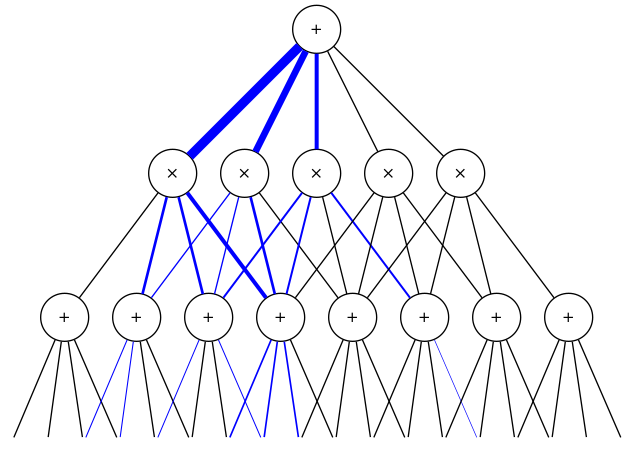
\includegraphics[scale=0.325]{graphs/softgrad.png}
  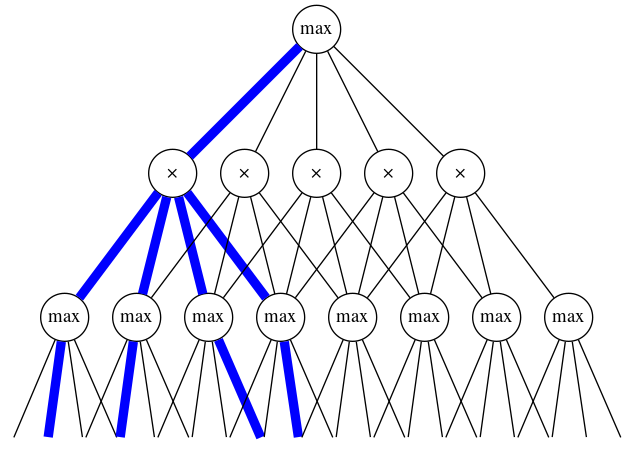
\includegraphics[scale=0.325]{graphs/hardgrad.png}
  \caption{Signal difference between soft and hard derivation.\label{fig:soft_hard_diff}}
\end{figure}

\autoref{fig:soft_hard_diff} gives a visual representation of the difference between soft and hard
derivation in gradient descent. MPNs preserve the signal, as the resulting gradient is constant.

To compute the hard derivatives of an SPN, we take its MPN and find its derivatives in a similar
way as in soft derivation. Let $M$ be an MPN\@. We shall call $W$ the multiset of weights that a
forward pass through $M$ visits. The value of $M$ is $M(X)=\prod_{w_i\in W}w_i^{c_i}$, where $c_i$
is the number of times $w_i$ appears in $W$. We can then take the logarithm of the MPN to end up
with a friendlier expression.

\begin{equation*}
  \ddspn{\log M}{w_{n,j}}=\ddspn{}{w_{n,j}}\log\left(\prod_{w_i\in W}w_i^{c_i}\right)=
    \frac{1}{\prod_{w_i\in W}w_i^{c_i}}\cdot c_{n,j}w_{n,j}^{c_{n,j}-1}\cdot\prod_{w_i\in
      W\setminus\{w_{n,j}\}}w_i^{c_i}
\end{equation*}

If we assume that weights are strictly positive, the resulting expression results in the final
hard derivative

\begin{equation}
  \ddspn{\log M}{w_{n,j}}=c_{n,j}\frac{w_{n,j}^{c_{n,j}-1}}{w_{n,j}^{c_{n,j}}}=
    \frac{c_{n,j}}{w_{n,j}}.\label{eq:hard_weight_update}
\end{equation}

Although not needed for the gradient, we can also compute the derivative in each internal node. The
process is similar to soft derivation. There is no change for parent product nodes. For parent max
nodes, we sum only contributions where $w_{n,j}\in W$.

\begin{equation}
  \ddspn{M}{M_j}=\sum_{\substack{n\in\Pa(j)\\n:\text{ max}}}
    \begin{cases}
      w_{k,n}\ddspn{M}{M_k} & \text{if $w_{k,n}\in W$}\\
      0 & \text{otherwise}
    \end{cases}
    + \sum_{\substack{n\in\Pa(j)\\n:\text{ product}}}\ddspn{M}{M_n}\prod_{k\in\Ch(n)\setminus\{j\}}M_k
\end{equation}

In summary, the derivatives of an SPN with respect to its internal nodes take values according
to~\autoref{tab:derivatives_spn}. The gradient components are shown
in~\autoref{tab:derivatives_weight}.

\begin{table}[h]
  \centering
  \begin{tabular}{l|l}
    \hline
    \multicolumn{1}{c}{\bfseries Inference} & \multicolumn{1}{c}{\bfseries Partial derivatives wrt
    internal node $j$}\\
    \hline & \\
    \textbf{Soft} & \(\displaystyle \ddspn{S}{S_j}=\sum_{\substack{n\in\Pa(j)\\n:\text{ sum}}}w_{n,j}
      \ddspn{S}{S_n}+\sum_{\substack{n\in\Pa(j)\\n:\text{ product}}}\ddspn{S}{S_n}\prod_{k\in\Ch(n)
      \setminus\{j\}}S_k\) \\
    & \\
    \textbf{Hard} & \(\displaystyle
        \ddspn{M}{M_j}=\sum_{\substack{n\in\Pa(j)\\n:\text{ max}}}
        \begin{cases}
          w_{k,n}\ddspn{M}{M_k} & \text{if $w_{k,n}\in W$,}\\
          0 & \text{otherwise.}
        \end{cases}
        + \sum_{\substack{n\in\Pa(j)\\n:\text{ product}}}\ddspn{M}{M_n}\prod_{k\in\Ch(n)\setminus\{j\}}M_k
      \) \\
      & \\
    \hline
  \end{tabular}
  \caption{Partial derivatives for the SPN wrt internal nodes.\label{tab:derivatives_spn}}
\end{table}

\begin{table}[h]
  \centering
  \begin{tabular}{l|c}
    \hline
    \multicolumn{1}{c}{\bfseries Inference} & \multicolumn{1}{c}{\bfseries Partial derivatives wrt
      weight $w_{n,j}$}\\
    \hline & \\
    \textbf{Soft} & \(\displaystyle \ddspn{S}{w_{n,j}} = S_j\ddspn{S}{S_n} \) \\
    & \\
    \textbf{Hard} & \(\displaystyle \ddspn{M}{w_{n,j}} = M_j\ddspn{M}{M_n} \) \\
    & \\
    \hline
  \end{tabular}
  \caption{Partial derivatives for the SPN wrt weights.\label{tab:derivatives_weight}}
\end{table}

\section{Generative gradient descent}

Once computed all derivatives, we update each node with the resulting gradient component. For
generative gradient descent, where we are learning a joint probability distribution $P(X,Y)$, our
objective is to find the gradient of the log-likelihood

\begin{equation*}
  \ddspn{}{W}\log P(X,Y)=\ddspn{}{W}\log S(X,Y)=\frac{1}{S(X,Y)}\ddspn{S}{W}(X,Y)\propto
    \ddspn{S}{W}(X,Y).
\end{equation*}

Since the gradient is proportional to the derivative of the weights, our weight update becomes

\begin{equation*}
  \Delta w_{n,j}=\eta\ddspn{S}{w_{n,j}}(X, Y),
\end{equation*}

where $\eta$ is the learning rate. An L2 regularization factor can be added to the expression
above, leaving us with the final generative gradient descent weight update

\begin{equation}\label{eq:gen_weight_update}
  \Delta w_{n,j}=\eta\ddspn{S}{w_{n,j}}(X, Y)-2\lambda w_{n,j},
\end{equation}

where $\lambda$ is the regularization constant. We call this soft generative gradient descent. It
is now easy to visualize why gradient diffusion occurs with soft derivation. Component
$\iddspn{S}{w_{n,j}}$ depends on partial derivative $\iddspn{S}{S_n}$. Assuming normalized weights,
the root node derivative $\iddspn{S}{S}=1$ and each subsequent descendant node becomes smaller and
smaller.

Weight update for hard derivation comes directly from~\autoref{eq:hard_weight_update}. Since we are
interested in the log-likelihood of the joint distribution

\begin{equation*}
  \ddspn{}{W}\log P(X,Y)=\ddspn{}{W}\log M(X,Y),
\end{equation*}

we get, for each component $w_{n,j}$, the weight update

\begin{equation*}
  \Delta w_{n,j}=\eta\frac{c_{n,j}}{w_{n,j}}.
\end{equation*}

In a similar fashion to soft generative gradient descent, we can apply L2 regularization to each
weight update.

\begin{equation}
  \Delta w_{n,j}=\eta\frac{c_{n,j}}{w_{n,j}}-2\lambda w_{n,j}
\end{equation}

So for generative gradient descent we get the following weight updates.

\begin{table}[h]
  \centering
  \begin{tabular}{l|l}
    \hline
    \multicolumn{1}{c}{\bfseries Inference} & \multicolumn{1}{c}{\bfseries Weight updates}\\
    \hline & \\
    \textbf{Soft} & \(\displaystyle \Delta w_{n,j}=\eta\ddspn{S}{w_{n,j}}(X, Y)-2\lambda w_{n,j} \) \\
    & \\
    \textbf{Hard} & \(\displaystyle \Delta w_{n,j}=\eta\frac{c_{n,j}}{w_{n,j}}-2\lambda w_{n,j} \) \\
    & \\
    \hline
  \end{tabular}
  \caption{Generative gradient descent weight updates with L2
    regularization.\label{tab:generative_weight_updates}}
\end{table}



\section{Discriminative gradient descent}


